../preamble/preamble.tex

\addbibresource{main.bib}

\newcommand\fullsum{\sum\limits_{n=1}^{N} \sum\limits_{m=1}^{M}}
\newcommand\fullphase{\omega_{nm}t + \vec \kappa_{nm}\vec r_0 + \psi_{nm}}

\title{Черновик статьи \\ \textbf{Моделирование акустического волнографа на
течении}}
\author{Понур К.А.}
\begin{document}

\maketitle

\section*{Орбитальные скорости}%
\label{sec:orbital_nye_skorosti}

Рассмотрим задачу нахождения орбитальных скоростей частиц на морской
поверхности.

Поле возвышений \where*{$\zeta$}{поле возвышений} представим в виде
\begin{equation}
    \label{eq:surface3d_default}
    \zeta(\vec r_0,t) = \fullsum A_n(\vec \kappa_{nm}) \cos(\fullphase),    \\
\end{equation}
где \where{$\vec \kappa$}{двумерный волновой вектор},  
$\vec r_0 = (x_0, y_0)$, $\vec r = (x, y)$, 
\where{$\psi_{nm}$}{случайная фаза равномерно распределенная в интервале от $0$ до $2 \pi$}, 

\where{$A_n (\vec \kappa_n)$}{комплексная амплитуда гармоники с волновым
вектором}
$\vec \kappa_n$ и временной частотой
\where*{$\omega_n(\kappa_{nm})$}{дисперсионное соотношение}.



Известно что в глубоком море
поверхностные частицы на волнах описывают окружность (см. \cite{shuleykin}).
Следовательно саму волну правильнее описывать параметрическим уравнением
трохоиды (см. \cite{nouguier})

\begin{equation}
    \begin{gathered}
        \label{eq:surface3d_cwm}
        x(\vec r,t) = x_0 - \fullsum A_n(\vec \kappa_{nm})\frac{\vec \kappa_x}{\kappa}        \sin(\fullphase)\\
        y(\vec r,t) = y_0 - \fullsum A_n(\vec \kappa_{nm}) \frac{\vec \kappa_y}{\kappa}
        \sin(\fullphase)\\
        z(\vec r,t) = \fullsum
        A_n(\vec \kappa_{nm}) \cdot \cos(\fullphase)    \\
    \end{gathered}
\end{equation}

Дифференцируя \eqref{eq:surface3d_cwm} получаем выражения для
проекций орбитальных
скоростей 
\begin{equation}
    \begin{gathered}
        \label{eq:orbital_velocity}
        v_x(\vec r, t)  = \pdv{x}{t} = - \fullsum \omega_n(\kappa_{nm}) A_n(\vec
        \kappa_{nm}) \frac{\vec \kappa_x}{\kappa} \cos(\fullphase) \\
        v_y (\vec r, t) = \pdv{y}{t} = - \fullsum \omega_n(\kappa_{nm}) A_n(\vec
        \kappa_{nm}) \frac{\vec \kappa_y}{\kappa}\cos(\fullphase) \\
        v_z (\vec r, t) = \pdv{\zeta}{t} = - \fullsum \omega_n(\kappa_{nm})
        A_n(\vec \kappa_{nm})
        \sin(\fullphase)
    \end{gathered}
\end{equation}




\begin{figure}[h]
\centering
\makeatletter
    \@for\i:={1,2,3,4}\do{
    \begin{subfigure}{0.45\textwidth}
        \centering
        \includegraphics[width=\linewidth, page=\i]{figs/cwm_demo}
        \subcaption{}
        \label{subfig:cwm_demo\i}
    \end{subfigure}
}

\label{fig:cwm_demo}
\caption{
    Сравнение характеристик заостренной и обычной поверхностей на примере одной
    синусоиды (эффект заострения усилен для наглядности): \\
    \subref{subfig:cwm_demo1} поле высот;
    \subref{subfig:cwm_demo2} поле полных наклонов;
    \subref{subfig:cwm_demo3} поле вертикальных орбитальных скоростей;
    \subref{subfig:cwm_demo4} поле горизонтальных орбитальных скоростей;
}
\makeatother
\end{figure}




\begin{figure}[h]
\centering
\makeatletter
    \@for\i:={1,2,3,4}\do{
    \begin{subfigure}{0.45\textwidth}
        \centering
        \includegraphics[width=\linewidth, ]{example-image-a}
        %\includegraphics[width=\linewidth, page=\i]{figs/cwm_demo}
        \subcaption{}
        \label{subfig:cwm_modeling\i}
    \end{subfigure}
    %\hfill
}

\label{fig:cwm_modeling}
\caption{
    Сравнение основных характеристик реализаций заостренной и обычной
    морских поверхностей: \\
    \subref{subfig:cwm_modeling1} поле высот;
    \subref{subfig:cwm_modeling2} поле полных наклонов;
    \subref{subfig:cwm_modeling3} поле вертикальных орбитальных скоростей;
    \subref{subfig:cwm_modeling4} поле горизонтальных орбитальных скоростей;
}
\makeatother
\end{figure}
%%Здесь начинается не понятный для меня момент. Шулейкин в \cite{shuleykin} при
%выводе орбитальных скоростей пользуется трохоидальной моделью поверхности, т.е.
%фактически орбитальные скорости \eqref{eq:orbital_velocity} были изначально
%получены для заостренной морской поверхности. 

%Не получается ли у нас так, что для обычной (синусоидальной поверхности)
%горизонтальная орбитальных скоростей нет как следствие отсутствия вращения
%частицы, а частица двигается просто со скоростью распространения волны? %должна быть равна всегда скорости
%распространения волны?
%Если мы представим одну синусоиду и будем наблюдать за одной точкой на ней, то
%она будет перемещаться только по вертикальной оси со скоростью
%$\pdv{\zeta}{t}$, а поскольку производная  $\pdv{x}{t} = 0$

%Поэтому мы можем записать орбитальную скорость $v_{\perp}$ в плоскости азимута
%\begin{equation}
    %v_{\perp} = + \fullsum \omega_n(\kappa_{nm}) A_n(\vec \kappa_{nm}) \cos(\fullphase)
%\end{equation}

%Получаем выражения для орбитальных скоростей $v_x$ и $v_y$
 %\begin{equation}
    %\begin{gathered}
        %v_x = \dv[]{x_0}{t} = \cos \phi_0 \fullsum \omega_n(\kappa_{nm}) A_n(\vec
        %\kappa_{nm}) \cos(\fullphase) \\
        %v_y = \dv[]{y_0}{t} = \sin \phi_0 \fullsum \omega_n(\kappa_{nm}) A_n(\vec
        %\kappa_{nm})\cos(\fullphase), \\
    %\end{gathered}
%\end{equation}
%где \where{$\phi_0$}{направление распространения волнения}.

%Для трехмерного случая Пирсон \cite{pierson} представил решение линеаризованных
%уравнений движения для невязкой жидкости в лагранжевых координатах. Он показал,
%что в глубокой воде положение частиц на свободной поверхности задается
%параметрическим уравнением трохоиды


%\begin{equation}
    %\begin{gathered}
        %v_x(\vec r(t), t) = \dv[]{x}{t} = \pdv[]{x}{x_0}\dv{x_0}{t} + \pdv{x}{t} \\

        %%v_y = \dv[]{y}{t} = \pdv[]{y}{y_0}\dv{y_0}{t} + \pdv{y}{t}
    %\end{gathered}
%\end{equation}

%\newpage
%\bibliographystyle{gost2008}
%%\bibliography{main}
\newpage
\printbibliography
%%\printnomenclature[5em]
\end{document}

